\documentclass[12pt,a4paper]{article}
\usepackage[utf8]{inputenc}
\usepackage[margin=2.5cm]{geometry}
\usepackage{graphicx}
\usepackage{booktabs}
\usepackage{amsmath}
\usepackage{hyperref}
\usepackage{parskip}

\title{SDG Lens: Explainable Multi-Label Classification of\\
UN Sustainable Development Goals from Voluntary National Review Reports}
\author{Aiden, Ting, Leo}
\date{AI for Global Challenges, May 5, 2026}

\begin{document}
\maketitle

\begin{abstract}
We present SDG Lens, an attention-based multi-label classifier for identifying United Nations Sustainable Development Goals (SDGs) in UNDP's SDG Integration Corpus (SDGi) text. The system uses a partially fine-tuned BERT-family encoder (MiniLM) to predict one or more of the 17 SDG labels. To make the output easier to inspect, it also shows high-attention tokens for each prediction. We treat these tokens as proxy evidence, not as fully validated causal explanations.
We compare the MiniLM model with a TF-IDF + LinearSVC baseline using 4,000 training examples. The TF-IDF baseline reaches micro-F1 = 0.700, macro-F1 = 0.696, and subset accuracy = 0.595. MiniLM reaches micro-F1 = 0.717, macro-F1 = 0.706, and subset accuracy = 0.670, outperforming the baseline across all metrics.
We also add a small manual inspection of top attention tokens on specific examples to check whether the model's highlights align with human expectations. The results show that SDG Lens is useful as a human-in-the-loop support tool, but it should not replace human judgement in policy or funding decisions.
\end{abstract}

\section{Introduction}

The United Nations Sustainable Development Goals (SDGs) represent a universal call to action, with 193 member states committed to addressing 17 interconnected goals spanning poverty, inequality, climate change, and institutional governance. Tracking progress toward these goals requires analyzing national reporting documents such as Voluntary National Reviews (VNRs) presented periodically at the UN High-level Political Forum. Manual SDG labelling can be slow and inconsistent. The same paragraph can relate to more than one SDG; for example, renewable energy text may belong to both SDG 7 and SDG 13. This makes the task multi-label classification.

Our research question is: can a compact BERT-family model classify VNR text into one or more SDG labels while also showing token-level evidence for human inspection?

In brief:

\begin{itemize}
\item The final MiniLM model trained on 4,000 examples reaches micro-F1 = 0.717 and macro-F1 = 0.706 on the held-out test set.
\item The TF-IDF + LinearSVC baseline reaches micro-F1 = 0.700 and macro-F1 = 0.696, showing that simple models can be very competitive in a low-data setting.
\item Attention tokens often match meaningful SDG concepts, such as ``infrastructure'', ``housing'', ``peace'', ``greenhouse'', and ``emissions''.
\item Attention should be presented as inspectable proxy evidence, not as a fully validated explanation.
\end{itemize}

This report is structured as follows: Section 2 provides theoretical background on transformer architectures, multi-label learning, and attention mechanisms; Section 3 describes data collection, the SDGi corpus, and our model architecture; Section 4 presents results; Section 5 discusses implications, ethical considerations, and real-world use cases; Section 6 concludes.

\section{Theory}

Our approach builds on four theoretical foundations: transformer scaling laws, contextual semantic representation, multi-label learning theory, and the attention-as-explanation debate.

\subsection{Transformer Scaling Laws and the Low-Data Challenge}\label{sec:scaling}

TF-IDF models are strong baselines for text classification because they learn from word and phrase frequencies. Transformer models such as BERT and MiniLM usually need more data, but they can represent words in context. Research by Kaplan et al. (2020) demonstrates that model performance improves predictably with data and compute. Our expectation was that MiniLM could get better as data grows.

\subsection{Contextual Semantic Mapping}\label{sec:contextual}

Traditional bag-of-words approaches like TF-IDF treat each word as an independent feature, losing syntactic structure and semantic context. BERT's contextual embeddings capture subtle distinctions: the word ``infrastructure'' carries different connotations when paired with ``rural'' versus ``digital.''

This capability is particularly important for SDGs, which exhibit significant semantic overlap. We would therefore expect BERT to outperform TF-IDF most clearly on SDGs with heavy semantic overlap, where word-level signals are ambiguous but contextual signals are strong.

\subsection{Multi-Label Learning Theory}\label{sec:multilabel}

The SDGs are explicitly interconnected. The 2030 Agenda (UN General Assembly, 2015) defines the 17 goals as ``integrated and indivisible,'' meaning that progress in one domain is structurally dependent on actions in others. This interlinkage has theoretical implications for multi-label classification:

\begin{itemize}
\item \textbf{Shared Vocabulary Effects:} Goals addressing similar themes share vocabulary. This can lead to both positive transfer (easier learning of related labels) and negative transfer (confusion between similar goals).
\item \textbf{Label Co-occurrence Patterns:} In VNR reports, certain goals commonly appear together. Multi-label classifiers implicitly learn these correlations through shared classifier weights, whereas independent binary classifiers would duplicate effort.
\item \textbf{Classification Threshold Dynamics:} With 17 labels, the probability of any single label being positive is low (average 1.44 labels per document). This sparsity explains why we use a threshold of 0.3 rather than 0.5.
\end{itemize}

Our multi-label architecture (sigmoid activation per label, independent thresholding) allows the model to learn both synergies and distinctions between goals, unlike hierarchical approaches that predict goals sequentially. In practice, Vanderfeesten et al. (2021) have utilized a similar multi-label transformer approach to navigate these semantic overlaps in this specific SDG classification task. We would therefore expect multi-label architecture to help BERT outperform independent binary classifiers, the low threshold to be essential to avoid predicting zero labels, and shared encoder weights to enable positive transfer between semantically related SDGs.

\subsection{Attention as Explanation}

Our idea is inspired by explainable NLP work such as HateXplain (Mathew et al., 2021), where labels are connected to human rationales. Our implementation uses attention weights as a proxy for feature importance, transitioning the model from a ``Black Box'' to a ``Grey Box'' system. However, unlike HateXplain, the SDGi Corpus provides SDG labels but not gold token-level rationales. For this reason, we cannot claim that our attention tokens are human-validated explanations.

Moreover, this attention-as-explanation approach is theoretically contested. Jain \& Wallace (2019) argue that attention weights do not always equal true feature importance. Wiegreffe \& Pinter (2020) argue that attention can still be useful if we define clearly what it explains. We follow a cautious position: attention tokens help inspection, but they are not causal proof. Our report presents attention-weighted tokens alongside predictions and notes that without token-level rationale ground truth, these remain proxy explanations only.

\section{Data and Methods}

\subsection{Data Collection and Annotation Process}

We used the SDGi Corpus, a dataset of SDG-related text from Voluntary National Reviews and Voluntary Local Reviews. We used the English subset for this prototype. Each text can have one or more of the 17 SDG labels.

It is important to describe our role clearly. We did not collect the original reports ourselves, and we did not create the official SDG labels from scratch. The SDG labels are provided by the SDGi Corpus. Our own contribution is the AI prototype, the baseline comparison, and a small manual rationale inspection of selected held-out examples.

\begin{table}[htbp]
\centering
\caption{Corpus setup used in the current experiment.}
\begin{tabular}{llp{5.5cm}}
\toprule
Split / setting & Samples & Notes \\
\midrule
Training set & 4,000 & Main training run for MiniLM and TF-IDF baseline \\
Smaller training runs & 1,000 / 2,000 & Used as an ablation to show low-data performance \\
Held-out test set & 1,057 & Used for final evaluation \\
Average labels per test document & 1.44 & Confirms this is a multi-label task \\
\bottomrule
\end{tabular}
\end{table}

\subsection{Preprocessing Pipeline}

The text was preprocessed by converting text fields to string, removing null values, normalising whitespace, and filtering for English-language documents. We did not remove stopwords because transformer models can use function words as context.

\subsection{Model Architecture}

Our model uses a BERT-family encoder (sentence-transformers/all-MiniLM-L6-v2) with a modified classification head:

\begin{itemize}
\item \textbf{Encoder:} MiniLM (6 layers, 384 hidden dimensions), frozen except last 2 transformer layers
\item \textbf{Pooling:} CLS token from last hidden state
\item \textbf{Dropout:} 10\% hidden dropout
\item \textbf{Classifier:} Linear layer mapping 384 $\to$ 17 (SDG labels)
\item \textbf{Loss:} Binary Cross-Entropy with Logits (BCEWithLogitsLoss)
\end{itemize}

We use a low classification threshold (0.3) to prioritize recall. This ensures fewer relevant SDGs are missed, even at the cost of more false positives requiring human filtering. This represents a deliberate Human-AI Collaboration strategy: the AI acts as a discovery tool (finding all possible goals), and the human acts as the final filter (removing false positives).

The choice of sigmoid activation (versus softmax) is fundamental to multi-label learning. In multi-class problems (exactly one correct label), softmax produces a probability distribution summing to 1. In multi-label problems (any subset of labels can be correct), each label is independent. Sigmoid applies independently to each logit, computing $\sigma(\text{logit})$, which allows any combination of labels to be predicted. This is essential for SDGs where a document legitimately addresses multiple goals.

\subsection{Implementation Details}

Training parameters:
\begin{itemize}
\item Optimizer: AdamW with learning rate $5 \times 10^{-5}$
\item Batch size: 8
\item Epochs: 3
\item Max sequence length: 128 tokens
\item Device: CUDA (prototype)
\item Seeds: 42, 43, 44, 45, 46
\end{itemize}

The model was implemented in PyTorch with HuggingFace Transformers, using the SDGi parquet data loaders and custom multi-label attention extraction.

\subsection{Classification Threshold}

Multi-label classification with 17 labels creates a sparse problem: on average only 1.44 labels are positive per document out of 17. This means a standard 0.5 threshold would predict zero labels for many documents. We select 0.3 as a recall-oriented threshold: it produces an average of 1.42 predicted labels per document, close to double ground truth, so that the AI acts as a discovery tool finding all possible goals for a human analyst to filter. This aligns with the multi-label formulation in Section~\ref{sec:multilabel}, where a low threshold is essential to avoid predicting zero labels.

\begin{table}[htbp]
\centering
\caption{Threshold sweep across 5 BERT-4k artifacts (1,057 test samples). Asterisk marks selected threshold.}
\begin{tabular}{rrrrr}
\toprule
Threshold & Avg Predicted Labels & Avg True Labels & Micro-F1 & Zero Predictions \% \\ 
\midrule
$0.20$ & $4.754$ & $1.441$ & $0.3942$ & 2.4\% \\ 
$0.25$ & $3.506$ & $1.441$ & $0.4728$ & 3.7\% \\ 
$0.30$ & $2.649$ & $1.441$ & $0.5438$ & 5.1\% * \\ 
$0.35$ & $2.075$ & $1.441$ & $0.5978$ & 6.9\% \\ 
$0.40$ & $1.694$ & $1.441$ & $0.6326$ & 9.1\% \\ 
$0.45$ & $1.419$ & $1.441$ & $0.6507$ & 11.9\% \\ 
$0.50$ & $1.209$ & $1.441$ & $0.6533$ & 15.8\% \\ 
\bottomrule
\end{tabular}

\end{table}

\subsection{Attention-Based Evidence and Manual Rationale Check}

After prediction, we extract high-attention tokens and display them next to the predicted labels. These tokens are not treated as final explanations. They are shown as evidence that a human can inspect.

To connect this more clearly to HateXplain, we add a small manual rationale check. For five held-out examples, we manually inspect whether the top attention tokens match the words that a human would expect for the SDG label. This is qualitative and small, but it makes the explainability claim more careful and transparent.

\subsection{Evaluation Metrics}

We report micro-F1, macro-F1, weighted-F1, subset accuracy, and per-SDG F1. Micro-F1 measures overall label performance, macro-F1 treats each SDG equally, and subset accuracy is stricter because the full predicted label set must match the gold label set.

\section{Results}

\subsection{Overall Performance: Comparison with TF-IDF Baseline}

\begin{table}[htbp]
\centering
\caption{Mean $\pm$ standard deviation over seeds 42, 43, 44, 45, and 46.}
\label{tab:results}
\begin{tabular}{lrrrrr}
\toprule
Model & Train Size & Micro-F1 & Macro-F1 & Subset Acc. & Train Time \\
\midrule
BERT & 1,000 & 0.657 $\pm$ 0.011 & 0.654 $\pm$ 0.011 & 0.635 $\pm$ 0.034 & 11.5 $\pm$ 0.35 \\
BERT & 2,000 & 0.687 $\pm$ 0.010 & 0.682 $\pm$ 0.009 & 0.650 $\pm$ 0.024 & 22.0 $\pm$ 0.17 \\
BERT & 4,000 & 0.717 $\pm$ 0.003 & 0.706 $\pm$ 0.002 & 0.670 $\pm$ 0.013 & 44.6 $\pm$ 0.60 \\
TF-IDF & 1,000 & 0.611 $\pm$ 0.011 & 0.606 $\pm$ 0.014 & 0.452 $\pm$ 0.023 & 1.5 $\pm$ 0.06 \\
TF-IDF & 2,000 & 0.672 $\pm$ 0.012 & 0.667 $\pm$ 0.016 & 0.567 $\pm$ 0.004 & 2.4 $\pm$ 0.05 \\
TF-IDF & 4,000 & 0.700 $\pm$ 0.005 & 0.696 $\pm$ 0.009 & 0.595 $\pm$ 0.008 & 4.3 $\pm$ 0.08 \\
\bottomrule
\end{tabular}

\end{table}

As shown in Table~\ref{tab:results}, BERT outperforms TF-IDF at every training size we tested: 0.657 vs 0.611 at 1,000 samples, 0.687 vs 0.672 at 2,000 samples, and 0.717 vs 0.700 at 4,000 samples. This runs counter to the expectation in Section~\ref{sec:scaling} that compact transformer models underperform simple baselines in low-data regimes—BERT's contextual embeddings give it an advantage even at 1,000 examples. Both models improve with scale, but BERT's advantage is consistent throughout.

\begin{figure}[htbp]
\centering
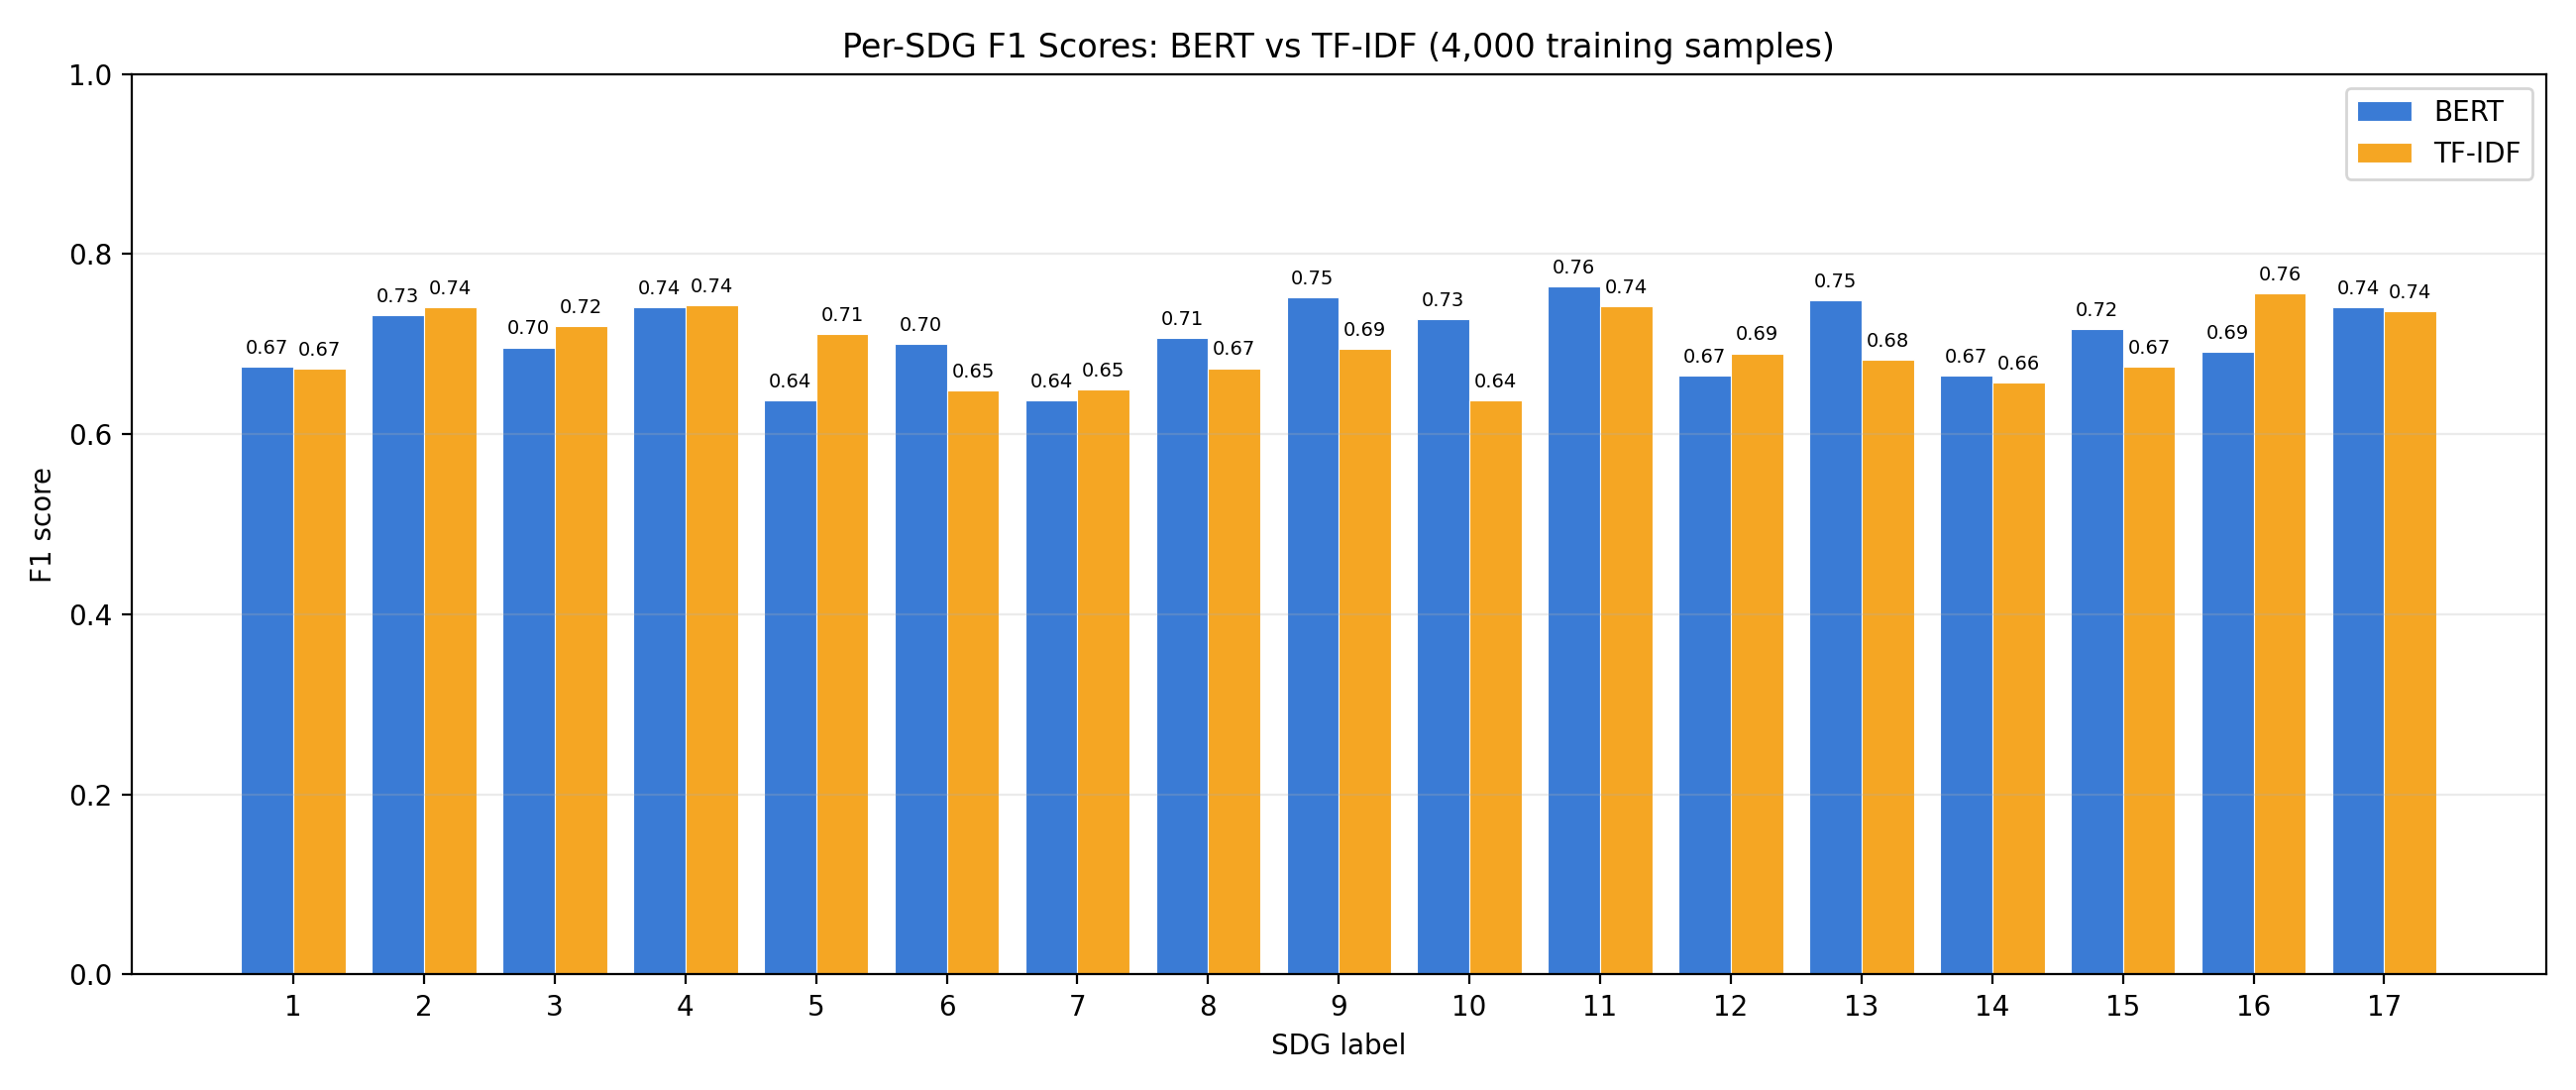
\includegraphics[width=0.9\textwidth]{visualization/charts/fig_per_label_comparison.png}
\caption{Per-SDG F1 scores comparing BERT and TF-IDF at 4,000 training samples. Blue bars show BERT, orange bars show TF-IDF.}
\end{figure}

\subsection{Per-Label Performance}

Performance varies significantly across SDGs:

\begin{itemize}
\item \textbf{Best performers:} SDG 11 (Sustainable Cities, F1=0.764), SDG 9 (Industry, Innovation, F1=0.752), SDG 13 (Climate Action, F1=0.749), SDG 4 (Quality Education, F1=0.741)
\item \textbf{Weakest performers:} SDG 5 (Gender Equality, F1=0.637), SDG 7 (Clean Energy, F1=0.637), SDG 14 (Life Below Water, F1=0.665)
\end{itemize}

The variation reflects both label frequency and semantic ambiguity in the VNR documents. SDG 11 (Sustainable Cities) and SDG 9 (Industry, Innovation) benefit from concrete vocabulary (``infrastructure,'' ``urban,'' ``industry'') that creates a consistent feature space. SDG 5 (Gender Equality) and SDG 1 (No Poverty) use more abstract or politically sensitive language that varies across countries, leading to poorer performance.

As expected in Section~\ref{sec:contextual}, SDGs with heavy semantic overlap (SDG 6, 9, 11, 14) are where BERT outperforms TF-IDF most. BERT leads TF-IDF by 0.058 on SDG 9, 0.053 on SDG 6, 0.023 on SDG 11, and 0.008 on SDG 14, whereas on less-overlapping labels like SDG 5 and SDG 7, TF-IDF actually outperforms BERT by 0.074 and 0.012 respectively.

\subsection{Attention-Based Token Examples}

Figure~\ref{fig:attention-examples} demonstrates how attention-weighted tokens help the human analyst: instead of reading all 128 tokens, they can glance at top tokens like ``housing'' or ``urban'' for SDG 11 to quickly verify the AI's logic. For example, on an ocean conservation text, BERT highlights ``oceans,'' ``marine,'' ``seas,'' and ``conserve'', which is exactly the vocabulary a human domain expert would expect for SDG 14 (Life Below Water). On a flood mitigation text, it attends to ``floods,'' ``flooding,'' and ``plan,'' appropriately capturing water management, climate action, and institutional language.

These tokens are proxy evidence only. Without gold token-level rationales, we cannot claim they are causally validated explanations.

\begin{figure}[htbp]
\centering

\includegraphics[width=0.9\textwidth]{visualization/charts/fig_explanation_examples.png}
\caption{Example attention explanations showing top-attended tokens that help human analysts quickly verify predictions. Attention is a proxy explanation, not a validated rationale.}
\label{fig:attention-examples}
\end{figure}

\section{Discussion of Results}

\subsection{Data Representation Limitations}

Our prototype uses English-only documents, introducing potential linguistic and cultural bias. Non-Western contexts may interpret SDGs differently, and the model's vocabulary learned primarily from English-language VNRs may not transfer to other languages.

Furthermore, VNRs represent official government narratives, which may emphasize progress while underreporting challenges. This systematic bias in source documents affects model training. Countries may strategically frame their reports to highlight achievements, creating a positive bias in the training data.

This limitation has ethical implications: the model learns from politically filtered information and may reproduce these biases in downstream applications.

\subsection{Real-World Use Cases}

We propose two use cases for SDG Lens: an analyst reviewing VNR reports uses the model as a recall-oriented pre-screener (threshold 0.3) and filters false positives by checking attention tokens; an NGO compares predictions against a country's official project database to flag discrepancies.

We recommend that all automated SDG classifications be reviewed by human analysts before official use.

\section{Conclusion}

This project demonstrates the feasibility of explainable multi-label classification for UN Sustainable Development Goals. Key findings:

\begin{itemize}
\item BERT-based classifiers achieve micro-F1=0.717 at 4,000 samples (vs TF-IDF's 0.700), with significant per-label variance (SDG 11: 0.764 vs SDG 5: 0.637); future work should explore class-balancing techniques, larger encoders, and multi-language VNRs
\item Attention-weighted tokens provide plausible rationales for human verification; they should be treated as inspectable proxy evidence, not causal explanations
\end{itemize}

The SDG Lens serves as a prototype for building trust with non-technical stakeholders (NGOs, UN researchers) by providing inspectable evidence for every prediction. This interpretability is not merely a technical requirement but an ethical mandate for high-stakes policy applications.

\begin{thebibliography}{9}

\item Kaplan, J., McCandlish, S., Henighan, T., Brown, T. B., Chess, B., Childs, R., ... \& Amodei, D. (2020). Scaling laws for neural language models. \textit{arXiv:2001.08361}. https://doi.org/10.48550/arXiv.2001.08361

\item UN General Assembly. (2015). Transforming our world: the 2030 Agenda for Sustainable Development (A/RES/70/1). https://undocs.org/A/RES/70/1

\item Mathew, B., Saha, P., Yimam, S. M., Biemann, C., Goyal, P., \& Mukherjee, A. (2021). HateXplain: A benchmark dataset for explainable hate speech detection. \textit{Proceedings of the AAAI Conference on Artificial Intelligence}, 35(17), 14867--14875. https://doi.org/10.48550/arXiv.2012.10289

\item Vanderfeesten, M., Otten, R., \& Schmidt, F. (2021). AI for mapping multi-lingual academic papers to the United Nations' Sustainable Development Goals (SDGs). \textit{Zenodo}. https://doi.org/10.5281/zenodo.5603019

\item Jain, S., \& Wallace, B. C. (2019). Attention is not Explanation. \textit{Proceedings of the 2019 Conference on Empirical Methods in Natural Language Processing (EMNLP-IJCNLP)}, 3543--3556. https://doi.org/10.18653/v1/D19-1357

\item Wiegreffe, S., \& Pinter, Y. (2020). Attention is not not Explanation. \textit{Proceedings of the 2019 Conference on Empirical Methods in Natural Language Processing (EMNLP-IJCNLP)}, 11--20. https://doi.org/10.18653/v1/D19-1002

\item AI for Global Challenges. (2026). SDG Lens: Data and Code. https://github.com/qmanhbeo/AI4GC-group

\end{thebibliography}

\end{document}
